% Options for packages loaded elsewhere
\PassOptionsToPackage{unicode}{hyperref}
\PassOptionsToPackage{hyphens}{url}
\documentclass[
  ignorenonframetext,
]{beamer}
\newif\ifbibliography
\usepackage{pgfpages}
\setbeamertemplate{caption}[numbered]
\setbeamertemplate{caption label separator}{: }
\setbeamercolor{caption name}{fg=normal text.fg}
\beamertemplatenavigationsymbolsempty
% remove section numbering
\setbeamertemplate{part page}{
  \centering
  \begin{beamercolorbox}[sep=16pt,center]{part title}
    \usebeamerfont{part title}\insertpart\par
  \end{beamercolorbox}
}
\setbeamertemplate{section page}{
  \centering
  \begin{beamercolorbox}[sep=12pt,center]{section title}
    \usebeamerfont{section title}\insertsection\par
  \end{beamercolorbox}
}
\setbeamertemplate{subsection page}{
  \centering
  \begin{beamercolorbox}[sep=8pt,center]{subsection title}
    \usebeamerfont{subsection title}\insertsubsection\par
  \end{beamercolorbox}
}
% Prevent slide breaks in the middle of a paragraph
\widowpenalties 1 10000
\raggedbottom
\AtBeginPart{
  \frame{\partpage}
}
\AtBeginSection{
  \ifbibliography
  \else
    \frame{\sectionpage}
  \fi
}
\AtBeginSubsection{
  \frame{\subsectionpage}
}
\usepackage{iftex}
\ifPDFTeX
  \usepackage[T1]{fontenc}
  \usepackage[utf8]{inputenc}
  \usepackage{textcomp} % provide euro and other symbols
\else % if luatex or xetex
  \usepackage{unicode-math} % this also loads fontspec
  \defaultfontfeatures{Scale=MatchLowercase}
  \defaultfontfeatures[\rmfamily]{Ligatures=TeX,Scale=1}
\fi
\usepackage{lmodern}
\usetheme[]{Montpellier}
\ifPDFTeX\else
  % xetex/luatex font selection
\fi
% Use upquote if available, for straight quotes in verbatim environments
\IfFileExists{upquote.sty}{\usepackage{upquote}}{}
\IfFileExists{microtype.sty}{% use microtype if available
  \usepackage[]{microtype}
  \UseMicrotypeSet[protrusion]{basicmath} % disable protrusion for tt fonts
}{}
\makeatletter
\@ifundefined{KOMAClassName}{% if non-KOMA class
  \IfFileExists{parskip.sty}{%
    \usepackage{parskip}
  }{% else
    \setlength{\parindent}{0pt}
    \setlength{\parskip}{6pt plus 2pt minus 1pt}}
}{% if KOMA class
  \KOMAoptions{parskip=half}}
\makeatother
\usepackage{color}
\usepackage{fancyvrb}
\newcommand{\VerbBar}{|}
\newcommand{\VERB}{\Verb[commandchars=\\\{\}]}
\DefineVerbatimEnvironment{Highlighting}{Verbatim}{commandchars=\\\{\}}
% Add ',fontsize=\small' for more characters per line
\usepackage{framed}
\definecolor{shadecolor}{RGB}{248,248,248}
\newenvironment{Shaded}{\begin{snugshade}}{\end{snugshade}}
\newcommand{\AlertTok}[1]{\textcolor[rgb]{0.94,0.16,0.16}{#1}}
\newcommand{\AnnotationTok}[1]{\textcolor[rgb]{0.56,0.35,0.01}{\textbf{\textit{#1}}}}
\newcommand{\AttributeTok}[1]{\textcolor[rgb]{0.13,0.29,0.53}{#1}}
\newcommand{\BaseNTok}[1]{\textcolor[rgb]{0.00,0.00,0.81}{#1}}
\newcommand{\BuiltInTok}[1]{#1}
\newcommand{\CharTok}[1]{\textcolor[rgb]{0.31,0.60,0.02}{#1}}
\newcommand{\CommentTok}[1]{\textcolor[rgb]{0.56,0.35,0.01}{\textit{#1}}}
\newcommand{\CommentVarTok}[1]{\textcolor[rgb]{0.56,0.35,0.01}{\textbf{\textit{#1}}}}
\newcommand{\ConstantTok}[1]{\textcolor[rgb]{0.56,0.35,0.01}{#1}}
\newcommand{\ControlFlowTok}[1]{\textcolor[rgb]{0.13,0.29,0.53}{\textbf{#1}}}
\newcommand{\DataTypeTok}[1]{\textcolor[rgb]{0.13,0.29,0.53}{#1}}
\newcommand{\DecValTok}[1]{\textcolor[rgb]{0.00,0.00,0.81}{#1}}
\newcommand{\DocumentationTok}[1]{\textcolor[rgb]{0.56,0.35,0.01}{\textbf{\textit{#1}}}}
\newcommand{\ErrorTok}[1]{\textcolor[rgb]{0.64,0.00,0.00}{\textbf{#1}}}
\newcommand{\ExtensionTok}[1]{#1}
\newcommand{\FloatTok}[1]{\textcolor[rgb]{0.00,0.00,0.81}{#1}}
\newcommand{\FunctionTok}[1]{\textcolor[rgb]{0.13,0.29,0.53}{\textbf{#1}}}
\newcommand{\ImportTok}[1]{#1}
\newcommand{\InformationTok}[1]{\textcolor[rgb]{0.56,0.35,0.01}{\textbf{\textit{#1}}}}
\newcommand{\KeywordTok}[1]{\textcolor[rgb]{0.13,0.29,0.53}{\textbf{#1}}}
\newcommand{\NormalTok}[1]{#1}
\newcommand{\OperatorTok}[1]{\textcolor[rgb]{0.81,0.36,0.00}{\textbf{#1}}}
\newcommand{\OtherTok}[1]{\textcolor[rgb]{0.56,0.35,0.01}{#1}}
\newcommand{\PreprocessorTok}[1]{\textcolor[rgb]{0.56,0.35,0.01}{\textit{#1}}}
\newcommand{\RegionMarkerTok}[1]{#1}
\newcommand{\SpecialCharTok}[1]{\textcolor[rgb]{0.81,0.36,0.00}{\textbf{#1}}}
\newcommand{\SpecialStringTok}[1]{\textcolor[rgb]{0.31,0.60,0.02}{#1}}
\newcommand{\StringTok}[1]{\textcolor[rgb]{0.31,0.60,0.02}{#1}}
\newcommand{\VariableTok}[1]{\textcolor[rgb]{0.00,0.00,0.00}{#1}}
\newcommand{\VerbatimStringTok}[1]{\textcolor[rgb]{0.31,0.60,0.02}{#1}}
\newcommand{\WarningTok}[1]{\textcolor[rgb]{0.56,0.35,0.01}{\textbf{\textit{#1}}}}
\usepackage{graphicx}
\makeatletter
\newsavebox\pandoc@box
\newcommand*\pandocbounded[1]{% scales image to fit in text height/width
  \sbox\pandoc@box{#1}%
  \Gscale@div\@tempa{\textheight}{\dimexpr\ht\pandoc@box+\dp\pandoc@box\relax}%
  \Gscale@div\@tempb{\linewidth}{\wd\pandoc@box}%
  \ifdim\@tempb\p@<\@tempa\p@\let\@tempa\@tempb\fi% select the smaller of both
  \ifdim\@tempa\p@<\p@\scalebox{\@tempa}{\usebox\pandoc@box}%
  \else\usebox{\pandoc@box}%
  \fi%
}
% Set default figure placement to htbp
\def\fps@figure{htbp}
\makeatother
\setlength{\emergencystretch}{3em} % prevent overfull lines
\providecommand{\tightlist}{%
  \setlength{\itemsep}{0pt}\setlength{\parskip}{0pt}}
%\documentclass[unicode,10pt]{beamer}% 'unicode'が必要
\usepackage{luatexja}% 日本語を使う場合は必須
%\usepackage[japanese]{babel}	
%\usefonttheme[onlymath]{serif}
%\usepackage[T1]{fontenc} %これを使うと、ギリシャ文字が出ない
%\usepackage{textcomp}
%\usepackage[scale=1.0]{tgheros} % Sans serif font
%\usepackage[scaled]{beramono} % Monospace font
%\usepackage{luatexja-otf}
%\renewcommand{\kanjifamilydefault}{\gtdefault}
%\usepackage[haranoaji]{luatexja-preset}

% スライド番号の表示 %%%%%%%%%%%%%%%%%%%
\makeatletter
\setbeamertemplate{footline}{%
  \leavevmode%
  \hbox{%
  \begin{beamercolorbox}[wd=.5\paperwidth,ht=2.25ex,dp=1ex,right]{date in head/foot}%
    \insertframenumber{} \hspace*{2ex} % new version without total frames
  \end{beamercolorbox}}%
  \vskip0pt%
}
\makeatother
% スライド番号の表示 %%%%%%%%%%%%%%%%%%%
\usepackage{float}
\usepackage{tabularray}
\usepackage[normalem]{ulem}
\usepackage{graphicx}
\usepackage{rotating}
\UseTblrLibrary{siunitx}
\NewTableCommand{\tinytableDefineColor}[3]{\definecolor{#1}{#2}{#3}}
\newcommand{\tinytableTabularrayUnderline}[1]{\underline{#1}}
\newcommand{\tinytableTabularrayStrikeout}[1]{\sout{#1}}
\usepackage{bookmark}
\IfFileExists{xurl.sty}{\usepackage{xurl}}{} % add URL line breaks if available
\urlstyle{same}
\hypersetup{
  hidelinks,
  pdfcreator={LaTeX via pandoc}}

\title{第5章: 多重回帰分析：OLS漸近特性}
\subtitle{Jeffrey Wooldridge (2016).\\
Introductory Econometrics: A Modern Approach\\
6rd ed.~Cengage Learning.}
\author{}
\date{\vspace{-2.5em}2026-01-23}

\begin{document}
\frame{\titlepage}

\section{準備}\label{ux6e96ux5099}

\begin{frame}[fragile]{必要なパッケージの読み込み}
\phantomsection\label{ux5fc5ux8981ux306aux30d1ux30c3ux30b1ux30fcux30b8ux306eux8aadux307fux8fbcux307f}
\begin{itemize}
\tightlist
\item
  \texttt{wooldridge}パッケージの読み込み
\end{itemize}

\begin{Shaded}
\begin{Highlighting}[]
\FunctionTok{library}\NormalTok{(wooldridge)}
\end{Highlighting}
\end{Shaded}
\end{frame}

\section{5-1 一致性 (Consistency)}\label{ux4e00ux81f4ux6027-consistency}

\begin{frame}{標本数と推定量}
\phantomsection\label{ux6a19ux672cux6570ux3068ux63a8ux5b9aux91cf}
\begin{itemize}
\tightlist
\item
  第4章までの性質（不偏性など）は、どのような標本サイズ \(n\)
  に対しても成立する\textbf{有限標本特性}（finite sample
  properties）であった。
\item
  第5章では、標本サイズ \(n\)
  が無限に大きくなったときの推定量の振る舞い、すなわち\textbf{漸近特性}（asymptotic
  properties）を扱う。
\item
  特に重要なのが、\textbf{一致性}（consistency）である。
\end{itemize}
\end{frame}

\begin{frame}{OLS推定量の一致性}
\phantomsection\label{olsux63a8ux5b9aux91cfux306eux4e00ux81f4ux6027}
\begin{itemize}
\tightlist
\item
  標本サイズ \(n\) が大きくなるにつれて、推定量 \(\hat{\beta}_j\)
  が真のパラメータ \(\beta_j\)
  に確率収束することを\textbf{一致性}という。
\end{itemize}

\[ \text{plim}(\hat{\beta}_j) = \beta_j \]

\begin{itemize}
\tightlist
\item
  仮定 MLR.1（線形性）〜
  MLR.4（ゼロ条件付き平均）が満たされれば、OLS推定量は一致性を持つ。
\item
  注：仮定 MLR.6（正規性）は一致性には不要である。
\end{itemize}
\end{frame}

\begin{frame}{不偏性と一致性の違い}
\phantomsection\label{ux4e0dux504fux6027ux3068ux4e00ux81f4ux6027ux306eux9055ux3044}
\begin{itemize}
\tightlist
\item
  \textbf{不偏性}:
  期待値が真の値に等しいこと（\(E(\hat{\beta}_j) = \beta_j\)）。サンプルサイズが小さくても成立する。
\item
  \textbf{一致性}:
  サンプルサイズが無限大の極限で、真の値に収束すること。
\item
  OLS推定量は、MLR.4 (\(E(u|x)=0\))
  が満たされれば不偏かつ一致推定量である。
\item
  しかし、少し弱い仮定（\(E(u)=0\) かつ
  \(\text{Cov}(x,u)=0\)）の下では、不偏ではないが一致性を持つ場合がある。
\end{itemize}
\end{frame}

\section{5-2
漸近正規性と大規模標本での推論}\label{ux6f38ux8fd1ux6b63ux898fux6027ux3068ux5927ux898fux6a21ux6a19ux672cux3067ux306eux63a8ux8ad6}

\begin{frame}{漸近正規性 (Asymptotic Normality)}
\phantomsection\label{ux6f38ux8fd1ux6b63ux898fux6027-asymptotic-normality}
\begin{itemize}
\tightlist
\item
  誤差項 \(u\) が正規分布に従わなくても（つまり MLR.6
  が満たされなくても）、標本サイズ \(n\) が十分に大きければ、OLS推定量
  \(\hat{\beta}_j\) の分布は近似的に正規分布に従う。
\end{itemize}

\[ \sqrt{n}(\hat{\beta}_j - \beta_j) \xrightarrow{d} \text{Normal}(0, \sigma^2 / a_j^2) \]

\begin{itemize}
\tightlist
\item
  これを\textbf{漸近正規性}と呼ぶ。
\item
  これにより、大規模標本（large
  sample）においては、誤差項の分布に関わらず
  t検定やF検定、信頼区間の構成が正当化される。
\end{itemize}
\end{frame}

\begin{frame}{実証分析における含意}
\phantomsection\label{ux5b9fux8a3cux5206ux6790ux306bux304aux3051ux308bux542bux610f}
\begin{itemize}
\tightlist
\item
  標本サイズが十分に大きい場合（例：数百以上）、データのヒストグラム（誤差項の分布）が正規分布に見えなくても、t値やp値を通常通り解釈してよい。
\item
  ただし、「十分に大きい」の基準はデータの性質による（極端な外れ値がある場合などは注意が必要）。
\end{itemize}
\end{frame}

\section{5-3
Rによるシミュレーション}\label{rux306bux3088ux308bux30b7ux30dfux30e5ux30ecux30fcux30b7ux30e7ux30f3}

\begin{frame}[fragile]{正規分布でない誤差項を持つモデル}
\phantomsection\label{ux6b63ux898fux5206ux5e03ux3067ux306aux3044ux8aa4ux5deeux9805ux3092ux6301ux3064ux30e2ux30c7ux30eb}
\begin{itemize}
\tightlist
\item
  誤差項が\textbf{一様分布}に従う場合のシミュレーションを行う。
\item
  真のモデル: \(y = 1 + 2x + u\), \(x \sim N(0, 1)\),
  \(u \sim \text{Uniform}(-\sqrt{3}, \sqrt{3})\) （分散は1）
\end{itemize}

\begin{Shaded}
\begin{Highlighting}[]
\FunctionTok{set.seed}\NormalTok{(}\DecValTok{123}\NormalTok{)}
\NormalTok{n\_sim }\OtherTok{\textless{}{-}} \DecValTok{1000}  \CommentTok{\# シミュレーション回数}
\NormalTok{beta1\_estimates }\OtherTok{\textless{}{-}} \FunctionTok{numeric}\NormalTok{(n\_sim)}
\NormalTok{n }\OtherTok{\textless{}{-}} \DecValTok{500}       \CommentTok{\# サンプルサイズ（比較的大きい）}

\ControlFlowTok{for}\NormalTok{(i }\ControlFlowTok{in} \DecValTok{1}\SpecialCharTok{:}\NormalTok{n\_sim)\{}
\NormalTok{  x }\OtherTok{\textless{}{-}} \FunctionTok{rnorm}\NormalTok{(n)}
\NormalTok{  u }\OtherTok{\textless{}{-}} \FunctionTok{runif}\NormalTok{(n, }\AttributeTok{min =} \SpecialCharTok{{-}}\FunctionTok{sqrt}\NormalTok{(}\DecValTok{3}\NormalTok{), }\AttributeTok{max =} \FunctionTok{sqrt}\NormalTok{(}\DecValTok{3}\NormalTok{)) }\CommentTok{\# 非正規}
\NormalTok{  y }\OtherTok{\textless{}{-}} \DecValTok{1} \SpecialCharTok{+} \DecValTok{2} \SpecialCharTok{*}\NormalTok{ x }\SpecialCharTok{+}\NormalTok{ u}
\NormalTok{  beta1\_estimates[i] }\OtherTok{\textless{}{-}} \FunctionTok{coef}\NormalTok{(}\FunctionTok{lm}\NormalTok{(y }\SpecialCharTok{\textasciitilde{}}\NormalTok{ x))[}\DecValTok{2}\NormalTok{]}
\NormalTok{\}}
\end{Highlighting}
\end{Shaded}
\end{frame}

\begin{frame}[fragile]{推定量の分布の確認}
\phantomsection\label{ux63a8ux5b9aux91cfux306eux5206ux5e03ux306eux78baux8a8d}
\begin{Shaded}
\begin{Highlighting}[]
\CommentTok{\# ヒストグラムと正規分布曲線の重ね書き}
\FunctionTok{hist}\NormalTok{(beta1\_estimates, }\AttributeTok{probability =} \ConstantTok{TRUE}\NormalTok{, }
     \AttributeTok{main =} \StringTok{"Distribution of OLS Estimator (n=500)"}\NormalTok{,}
     \AttributeTok{xlab =} \StringTok{"Estimated Beta1"}\NormalTok{)}
\FunctionTok{curve}\NormalTok{(}\FunctionTok{dnorm}\NormalTok{(x, }\AttributeTok{mean =} \DecValTok{2}\NormalTok{, }\AttributeTok{sd =} \FunctionTok{sd}\NormalTok{(beta1\_estimates)), }
      \AttributeTok{add =} \ConstantTok{TRUE}\NormalTok{, }\AttributeTok{col =} \StringTok{"red"}\NormalTok{, }\AttributeTok{lwd =} \DecValTok{2}\NormalTok{)}
\end{Highlighting}
\end{Shaded}

\pandocbounded{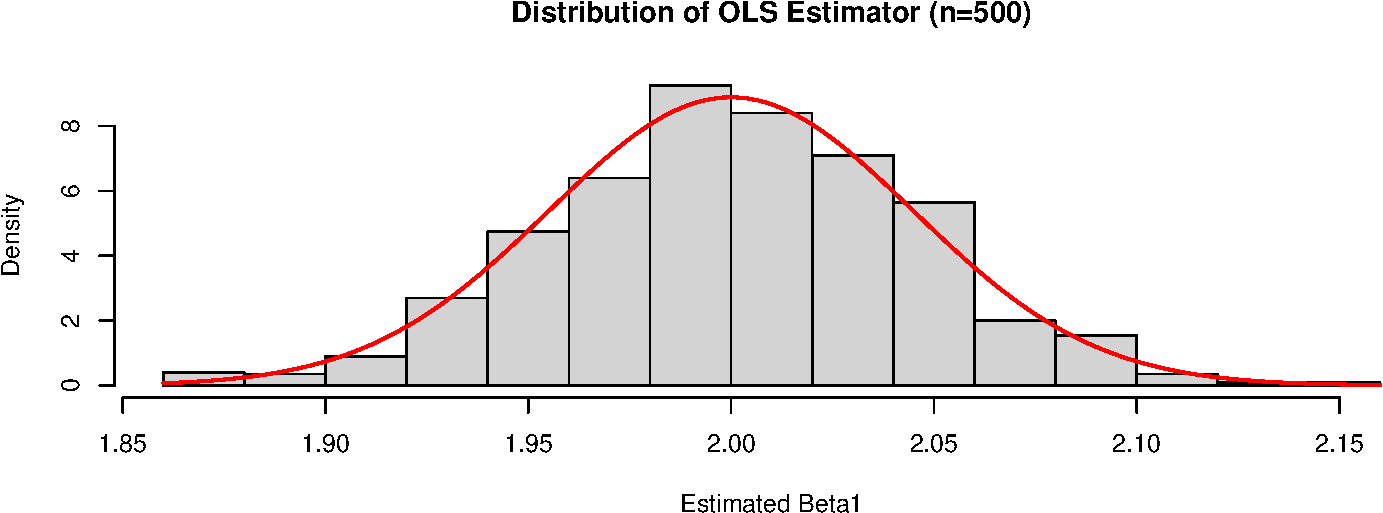
\includegraphics[keepaspectratio]{Wooldridge05_files/figure-beamer/unnamed-chunk-2-1.pdf}}

\begin{itemize}
\tightlist
\item
  誤差項は一様分布だが、推定量の分布は綺麗な正規分布（ベル型）になっていることがわかる。
\end{itemize}
\end{frame}

\section{5-4 大規模標本でのラグランジュ乗数検定
(LM検定)}\label{ux5927ux898fux6a21ux6a19ux672cux3067ux306eux30e9ux30b0ux30e9ux30f3ux30b8ux30e5ux4e57ux6570ux691cux5b9a-lmux691cux5b9a}

\begin{frame}{LM検定 (Lagrange Multiplier Statistic)}
\phantomsection\label{lmux691cux5b9a-lagrange-multiplier-statistic}
\begin{itemize}
\tightlist
\item
  複数の制約に関する検定として、F検定の代わりに使用されることがある。
\item
  特に、\textbf{制約付きモデル}（Restricted
  Model）のみを推定すればよいため、制約なしモデルの推定が困難な場合に便利である。
\item
  大規模標本において、LM統計量はカイ二乗分布 \(\chi^2_q\) に従う（\(q\)
  は制約の数）。
\end{itemize}
\end{frame}

\begin{frame}{LM検定の手順}
\phantomsection\label{lmux691cux5b9aux306eux624bux9806}
\begin{enumerate}
\tightlist
\item
  制約付きモデル（\(H_0\) を課したモデル）を推定し、残差 \(\tilde{u}\)
  を保存する。
\item
  残差 \(\tilde{u}\)
  を、制約なしモデルの\textbf{すべての}独立変数で回帰する（補助回帰）。
\item
  この補助回帰の決定係数 \(R^2_{\tilde{u}}\) を取得する。
\item
  \(LM = n \cdot R^2_{\tilde{u}}\) を計算する。
\item
  自由度 \(q\) のカイ二乗分布と比較してp値を求める。
\end{enumerate}
\end{frame}

\begin{frame}[fragile]{LM検定の例 (\texttt{crime1})}
\phantomsection\label{lmux691cux5b9aux306eux4f8b-crime1}
\begin{itemize}
\tightlist
\item
  \(H_0: \beta_{\text{avgsen}} = 0, \beta_{\text{tottime}} = 0\)
  （刑罰の厳しさは犯罪率に影響しない）
\end{itemize}

\begin{Shaded}
\begin{Highlighting}[]
\FunctionTok{data}\NormalTok{(crime1)}
\NormalTok{n }\OtherTok{\textless{}{-}} \FunctionTok{nrow}\NormalTok{(crime1)}
\CommentTok{\# 1. 制約付きモデル（刑罰変数なし）}
\NormalTok{model\_r }\OtherTok{\textless{}{-}} \FunctionTok{lm}\NormalTok{(narr86 }\SpecialCharTok{\textasciitilde{}}\NormalTok{ pcnv }\SpecialCharTok{+}\NormalTok{ ptime86 }\SpecialCharTok{+}\NormalTok{ qemp86, }
              \AttributeTok{data =}\NormalTok{ crime1)}
\NormalTok{u\_tilde }\OtherTok{\textless{}{-}} \FunctionTok{resid}\NormalTok{(model\_r)}

\CommentTok{\# 2. 補助回帰（残差をすべての変数で回帰）}
\CommentTok{\# avgsen, tottime を追加}
\NormalTok{model\_aux }\OtherTok{\textless{}{-}} \FunctionTok{lm}\NormalTok{(u\_tilde }\SpecialCharTok{\textasciitilde{}}\NormalTok{ pcnv }\SpecialCharTok{+}\NormalTok{ ptime86 }\SpecialCharTok{+}\NormalTok{ qemp86 }\SpecialCharTok{+} 
\NormalTok{                avgsen }\SpecialCharTok{+}\NormalTok{ tottime, }\AttributeTok{data =}\NormalTok{ crime1)}
\end{Highlighting}
\end{Shaded}
\end{frame}

\begin{frame}{}
\phantomsection\label{section}
\scriptsize

\begin{table}
\centering
\begin{talltblr}[         %% tabularray outer open
entry=none,label=none,
note{}={+ p < 0.1, * p < 0.05, ** p < 0.01, *** p < 0.001},
]                     %% tabularray outer close
{                     %% tabularray inner open
colspec={Q[]Q[]Q[]},
hline{2}={1-3}{solid, black, 0.05em},
hline{14}={1-3}{solid, black, 0.05em},
hline{1}={1-3}{solid, black, 0.1em},
hline{17}={1-3}{solid, black, 0.1em},
column{2-3}={}{halign=c},
column{1}={}{halign=l},
}                     %% tabularray inner close
& Restricted Model & Auxiliary Regression \\
(Intercept) & 0.712*** & -0.006 \\
& (0.033) & (0.033) \\
pcnv & -0.150*** & -0.001 \\
& (0.041) & (0.041) \\
ptime86 & -0.034*** & -0.005 \\
& (0.009) & (0.009) \\
qemp86 & -0.104*** & 0.001 \\
& (0.010) & (0.010) \\
avgsen &  & -0.007 \\
&  & (0.012) \\
tottime &  & 0.012 \\
&  & (0.010) \\
R2 & 0.041 & 0.001 \\
R2 Adj. & 0.040 & -0.000 \\
RMSE & 0.84 & 0.84 \\
\end{talltblr}
\end{table}
\end{frame}

\begin{frame}[fragile]{LM検定の計算}
\phantomsection\label{lmux691cux5b9aux306eux8a08ux7b97}
\begin{Shaded}
\begin{Highlighting}[]
\CommentTok{\# 3 \& 4. LM統計量の計算}
\NormalTok{lm\_stat }\OtherTok{\textless{}{-}}\NormalTok{ n }\SpecialCharTok{*} \FunctionTok{summary}\NormalTok{(model\_aux)}\SpecialCharTok{$}\NormalTok{r.squared}
\NormalTok{lm\_stat}
\end{Highlighting}
\end{Shaded}

\begin{verbatim}
## [1] 4.070729
\end{verbatim}
\end{frame}

\begin{frame}[fragile]{LM検定の判定}
\phantomsection\label{lmux691cux5b9aux306eux5224ux5b9a}
\begin{Shaded}
\begin{Highlighting}[]
\CommentTok{\# 5. p値の計算 (自由度 q = 2)}
\NormalTok{p\_value }\OtherTok{\textless{}{-}} \DecValTok{1} \SpecialCharTok{{-}} \FunctionTok{pchisq}\NormalTok{(lm\_stat, }\AttributeTok{df =} \DecValTok{2}\NormalTok{)}
\NormalTok{p\_value}
\end{Highlighting}
\end{Shaded}

\begin{verbatim}
## [1] 0.1306328
\end{verbatim}

\begin{itemize}
\tightlist
\item
  p値が \(0.05\) より大きければ、帰無仮説を棄却できない。
\item
  F検定の結果と（漸近的に）類似するはずである。
\end{itemize}
\end{frame}

\section{まとめ}\label{ux307eux3068ux3081}

\begin{frame}{まとめ}
\phantomsection\label{ux307eux3068ux3081-1}
\begin{itemize}
\tightlist
\item
  OLS推定量は、標本サイズが大きくなると真の値に確率収束する（\textbf{一致性}）。
\item
  誤差項が正規分布でなくても、標本サイズが十分に大きければ、OLS推定量は近似的に正規分布に従う（\textbf{漸近正規性}）。
\item
  これにより、大規模標本では通常のt検定やF検定が妥当となる。
\item
  LM検定は、大規模標本においてF検定の代替として利用できる（補助回帰を用いる）。
\end{itemize}
\end{frame}

\end{document}
